\documentclass[a4paper]{article}

\documentclass[a4paper]{article}
\usepackage[utf8]{inputenc}
\usepackage[spanish, es-tabla, es-noshorthands]{babel}
\usepackage[table,xcdraw]{xcolor}
\usepackage[a4paper, footnotesep = 1cm, width=20cm, top=2.5cm, height=25cm, textwidth=18cm, textheight=25cm]{geometry}
%\geometry{showframe}

\usepackage{tikz}
\usepackage{amsmath}
\usepackage{amsfonts}
\usepackage{amssymb}
\usepackage{float}
\usepackage{graphicx}
\usepackage{caption}
\usepackage{subcaption}
\usepackage{multicol}
\usepackage{multirow}
\setlength{\doublerulesep}{\arrayrulewidth}
\usepackage{booktabs}

\usepackage{hyperref}
\hypersetup{
    colorlinks=true,
    linkcolor=blue,
    filecolor=magenta,      
    urlcolor=blue,
    citecolor=blue,    
}

\newcommand{\quotes}[1]{``#1''}
\usepackage{array}
\newcolumntype{C}[1]{>{\centering\let\newline\\\arraybackslash\hspace{0pt}}m{#1}}
\usepackage[american]{circuitikz}
\usetikzlibrary{calc}
\usepackage{fancyhdr}
\usepackage{units} 

\graphicspath{{../Ejercicio-1/}{../Ejercicio-2/}{../Ejercicio-3/}{../Ejercicio-4/}}

\pagestyle{fancy}
\fancyhf{}
\lhead{22.01 Teoría de Circuitos}
\rhead{Mechoulam, Lambertucci, Rodriguez Turco, Londero, Galdeman}
\rfoot{\centering \thepage}

\usepackage{float}
\usepackage{graphicx}

\usepackage[american voltage]{circuitikz}

\usepackage{amsmath}

\usepackage{xcolor}

\usepackage{caption}
\usepackage{subcaption}

\begin{document}

\subsection{Diseño del circuito}

En el siguiente punto se propuso como objetivo realizar un sensor de temperatura, valiéndose del uso del transistor LM35. Este dispositivo se caracteriza por entregar a la salida una tensión proporcional a la temperatura de la forma
\[
	V_{LM35} = 10 \frac{mV}{^{\circ}C} \ T
\]

Como se requiere que el circuito diseñado posea una tensión de salida de $ 0 \ V $ a $ 35 ^{\circ}C $ y $ 5 \ V $ a $ 45 ^{\circ}C $, se busca la ecuación de la recta que atraviese los puntos especificados. Es así que se obtiene que la tensión de salida viene dada por la siguiente ecuación:

\begin{equation}
	V_{o} = 50V_{LM35} - 17.5 \ V =  0.5 \frac{V}{^{\circ}C} \ T - 17.5 \ V
	\label{equ:sistema}
\end{equation}

Para lograr su funcionamiento, el fabricante especifica que el transistor debe ser alimentado con una tensión de entre $4 \ V$ y $20 \ V$. Es por ello que se decidió suministrarle a este dispositivo $10 \ V$ para utilizarlo. Además, por cuestiones de seguridad, se desea que el circuito no brinde una tensión de salida menor a $-1 \ V$ ni mayor a $6 \ V$. Esto se ahondará con mayor profundidad en los de diseño del modelo.

Luego se requiere que la tensión de salida del circuito responda de la siguiente forma frente a la tensión de salida del transistor.

\begin{figure}[H]
	\centering
	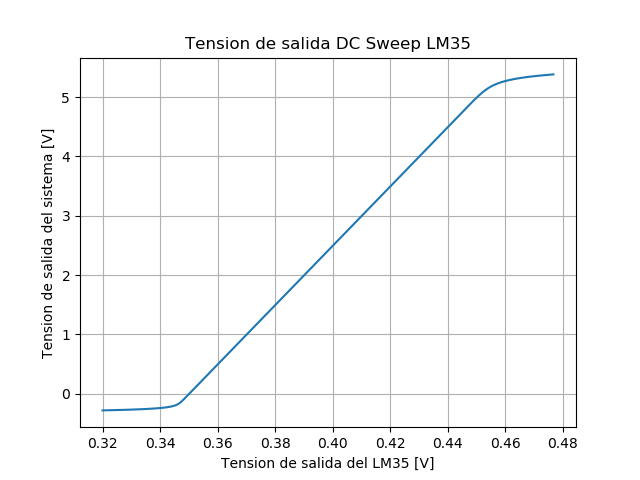
\includegraphics[width=0.8\textwidth]{Ejercicio6/Imagenes/SalidaVsVLM35.png}
\caption{Tensión de salida Vs. Tensión del LM35.}
	\label{fig:vout}
\end{figure}


\subsubsection{Primer modelo: inversor y restador}

En un principio, se decidió armar un circuito compuesto por tres diferentes etapas, las dos primeras compuestas cada una por un amplificador operacional TL072 y la final por un diodo zener DZ5V6-05. Cabe destacar que por cuestiones de especificación del fabricante, se decidió alimentar a ambos operacionales con $10 \ V$ y $-10 \ V$.

En la primer etapa se dispuso un amplificador inversor, tomando como tensión de entrada la de salida del transistor.

\begin{figure}[H]
\begin{center}
\begin{circuitikz}
	\node [op amp](A1){};
	\draw (A1.-) to[short] ++(-1,0) to[R, l = $R_5$, i^<=$I_{R5}$] ++(-2,0) to[short, -o] node[ocirc,label=left:$V_{LM35}$]{} ++(-1,0);
	\draw (A1.-) node[label=south:$V^-$]{};
	\draw (A1.+) node[label=south:$V^+$]{};
	\draw (A1.+) to[short] ++(-1,0) node[ground]{};
	\draw (A1.-) to[short] ++(0,1.5) to[R, l = $R_6$, i<=$I_{R6}$] ++(3,0) to[short] ++(0,-2);
	\draw (A1.out) to[short, -o] ++(2,0) node[ocirc,label=right:$V_{1}$]{};
\end{circuitikz}
\caption{Primera etapa del circuito.}
	\label{fig:cir1-M1}
\end{center}
\end{figure}

Planteando las siguientes ecuaciones:

\begin{equation*}
\left\{
\begin{aligned}
		& V_{LM35} = A_o \left( V^+ - V^- \right) =  A_o V^- \\
		& V_{LM35} - R_5 I_{R5} = V^- \\
		& V_1 - R_6 I_{R6} = V^- 
\end{aligned}
\right.
\end{equation*}

y sabiendo que $A_o \gg \frac{R_6}{R_5}$, se obtiene

\begin{equation}
	V_1 = -\frac{R_6}{R_5} \ V_{LM35}
	\label{equ:m1p1}
\end{equation}

siendo $V_1$ la tensión de salida de esta etapa.

En la segunda etapa, a diferencia de la primera, se utilizó un amplificador restador. Se decidió conectar al borne inversor del operacional la tensión $V_1$ y al una no inversor tensión de $- 10 \ V$, reutilizando la alimentación del operacional.

\begin{figure}[H]
\begin{center}
\begin{circuitikz}
	\node [op amp](A1){};
	\draw (A1.-) to[short] ++(-1,0) to[R, l_=$R_1$, i<_=$I_{R1}$] ++(-2,0) to[short, -o] node[ocirc,label=left:$V_{1}$]{} ++(-1,0);
	\draw (A1.-) node[label=south:$V^-$]{};
	\draw (A1.+) node[label=south:$V^+$]{};
	\draw (A1.+) to[short] ++(-1,0) to[R, l = $R_4$, i_>=$I_{R4}$] ++(0,-3) node[ground]{};
	\draw (A1.-) to[short] ++(0,1.5) to[R, l = $R_3$, i<=$I_{R3}$] ++(3,0) to[short] ++(0,-2);
	\draw (A1.out) to[short, -o] ++(2,0) node[ocirc,label=right:$V_{2}$]{};
	\draw (A1.+) to[short] ++(-1,0) to[R, l= $R_2$, i<_=$I_{R2}$] ++(-2,0) to[short, -o] node[ocirc,label=left:$-Vcc$]{} ++(-1,0);
\end{circuitikz}
	\caption{Segunda etapa del circuito.}
	\label{fig:cir2-M1}
\end{center}
\end{figure}

Aplicando el teorema de superposición, se puede obtener la transferencia de este circuito. De esta forma se compone por una parte sumadora y por otra restadora. Mientras que para la restadora, la transferencia se calcula de la misma forma que en (\ref{equ:m1p1}), para la sumadora se deben plantear:

\begin{equation*}
\left\{
\begin{aligned}
  		& V_2 = A_o \left( V^+ - V^- \right) =  A_o V^- \\
  		& V^- = V_2 \frac{R_1}{R_1 + R_3} \\
  		& V^+ = -Vcc \frac{R_4}{R_2 + R_4}
\end{aligned}
\right.
\end{equation*}

Es así que, sumando ambos resultados se obtiene

\begin{equation}
	V_2 = \frac{R_3}{R_2} \cdot \frac{R_2 // R_4}{R_1 // R_3} \left( -V_{CC} \right) \ - \ \frac{R_3}{R_1} V_1
	\label{equ:m1p2}
\end{equation}

Finalmente, la tercer etapa, consiste simplemente en una resistencia con un diodo zener en serie, cumpliendo la función de limitar la salida entre $-0.7 \ V$ y $5.6 \ V$. El objetivo de esta sección es simplemente limitar la tensión de salida, evitando que se encuentre por debajo de $-1 \ V$ y por encima de $6 \ V$.

\begin{figure}[H]
\begin{center}
\begin{circuitikz}
	\node [](v2){};
	\draw (v2) node[label=left:$V_2$]{} to[short, o-] ++ (0.5,0) to[R, l = $R_7$] ++ (2,0) to[open] ++(0,-2) node[ground](gnd){};
	\draw (gnd) to[zzDo, l_= $D$] ++(0,2);
	\draw (v2) to[open] ++(2.5,0) to[short, -o] ++(1,0) node[label=right:$V_o$](){};
	\end{circuitikz}
	\caption{Tercer etapa del circuito.}
	\label{fig:cir3}
\end{center}
\end{figure}

Es así como se observa al circuito final en la Figura (\ref{fig:cirfin-M1}).

\begin{figure}[H]
\hspace*{-2cm}
\begin{circuitikz}
	\node [op amp](A1){};
	\draw (A1.-) to[short] ++(-1,0) to[R, l = $R_5$] ++(-1.5,0) to[short, -o] node[ocirc,label=left:$V_{LM35}$]{} ++(-1,0);
	\draw (A1.+) to[short] ++(-1,0) node[ground]{};
	\draw (A1.-) to[short] ++(0,1.5) to[R, l = $R_6$] ++(2.5,0) to[short] ++(0,-2);

	\draw (A1.out) to[open] ++(4,-0.5) node [op amp](A2){};	
	\draw (A2.-) to[short] ++(-0.5,0) to[R, l_=$R_1$] ++(-1.5,0) to[short] (A1.out);
	\draw (A2.+) to[short] ++(0,0) to[R, l = $R_4$] ++(0,-3) node[ground]{};
	\draw (A2.-) to[short] ++(0,1.5) to[R, l = $R_3$] ++(2.5,0) to[short] ++(0,-2);
	\draw (A2.+) to[short] ++(-0.5,0) to[R, l= $R_2$] ++(-1.5,0) to[short, -o] node[ocirc,label=left:$-Vcc$]{} ++(-1,0);
	\draw (A2.out) to[short] ++ (0.5,0) to[R, l = $R_7$] ++ (1.5,0) to[open] ++(0,-2) node[ground](gnd){};
	\draw (gnd) to[zzDo, l_= $D$] ++(0,2);
	\draw (A2.out) to[open] ++(2,0) to[short, -o] ++(1,0) node[label=right:$V_o$](){};
	
	\end{circuitikz}
	\caption{Modelo final del circuito.}
	\label{fig:cirfin-M1}
\end{figure}

Se calcula la transferencia utilizando (\ref{equ:m1p1}) y (\ref{equ:m1p2}). Es así que se llega a
\begin{equation}
	V_{out} = \frac{R_3}{R_2} \cdot \frac{R_2 // R_4}{R_1 // R_3} \left( -V_{CC} \right) \ + \
	\frac{R_3}{R_1} \frac{R_6}{R_5} \ V_{LM35}
	\label{equ:transfm1}
\end{equation}

A la hora de seleccionar los valores de las resistencias, se pide:

\begin{equation*}
\left\{
\begin{aligned}
  		&	\frac{R_6}{R_5} = 5	\\
  		&	\frac{R_3}{R_1} = 10	\\
  		&	\frac{R_3}{R_2} = 1.75	\\
  		&	\frac{R_2 // R_4}{R_1 // R_3} = 1
\end{aligned}
\right.
\end{equation*}

Cumpliendo con esto y eligiendo arbitrariamente $R_6 = 5 \ k\Omega$ y $R_2 = 10 \ k\Omega$ se llega a los siguientes valores: $R_5 = 1 \ k\Omega$, $R_1 = 1.75 \ k\Omega$, $R_3 = 17.5 \ k\Omega$ y $R_4 = \frac{37}{7} \ k\Omega \approx 1.89 \ k\Omega$. De esta forma se consigue llegar a (\ref{equ:sistema}).

Por otro lado, para $R_7$ y debido a la función que cumple, para seleccionar un valor adecuado, se considera la máxima tensión que se puede obtener a la salida el operacional, $13.5 \ V$ en el peor caso, según el fabricante, y se asume una corriente de $0.5 \ mA$ para evitar que se sobre exija al operacional:

\begin{equation}
	R_7 = \frac{13.5 \ V \ - \ 5.6 \ V}{0.5 \ mA} = 15.8 \ k\Omega \approx 16 \ k\Omega
	\label{equ:rzener}
\end{equation}

Una vez establecido tanto la forma del circuito como sus componentes, se procedió a analizar simulaciones del mismo mediante el uso del programa LTSpice. En este, se valió del comando ``.step'' para analizar cada resistencia con una tolerancia del 5\%. Es por ello que se realiza un detenimiento en las resistencias $R_1$ y $R_4$.

\begin{figure}[H]
	\centering
	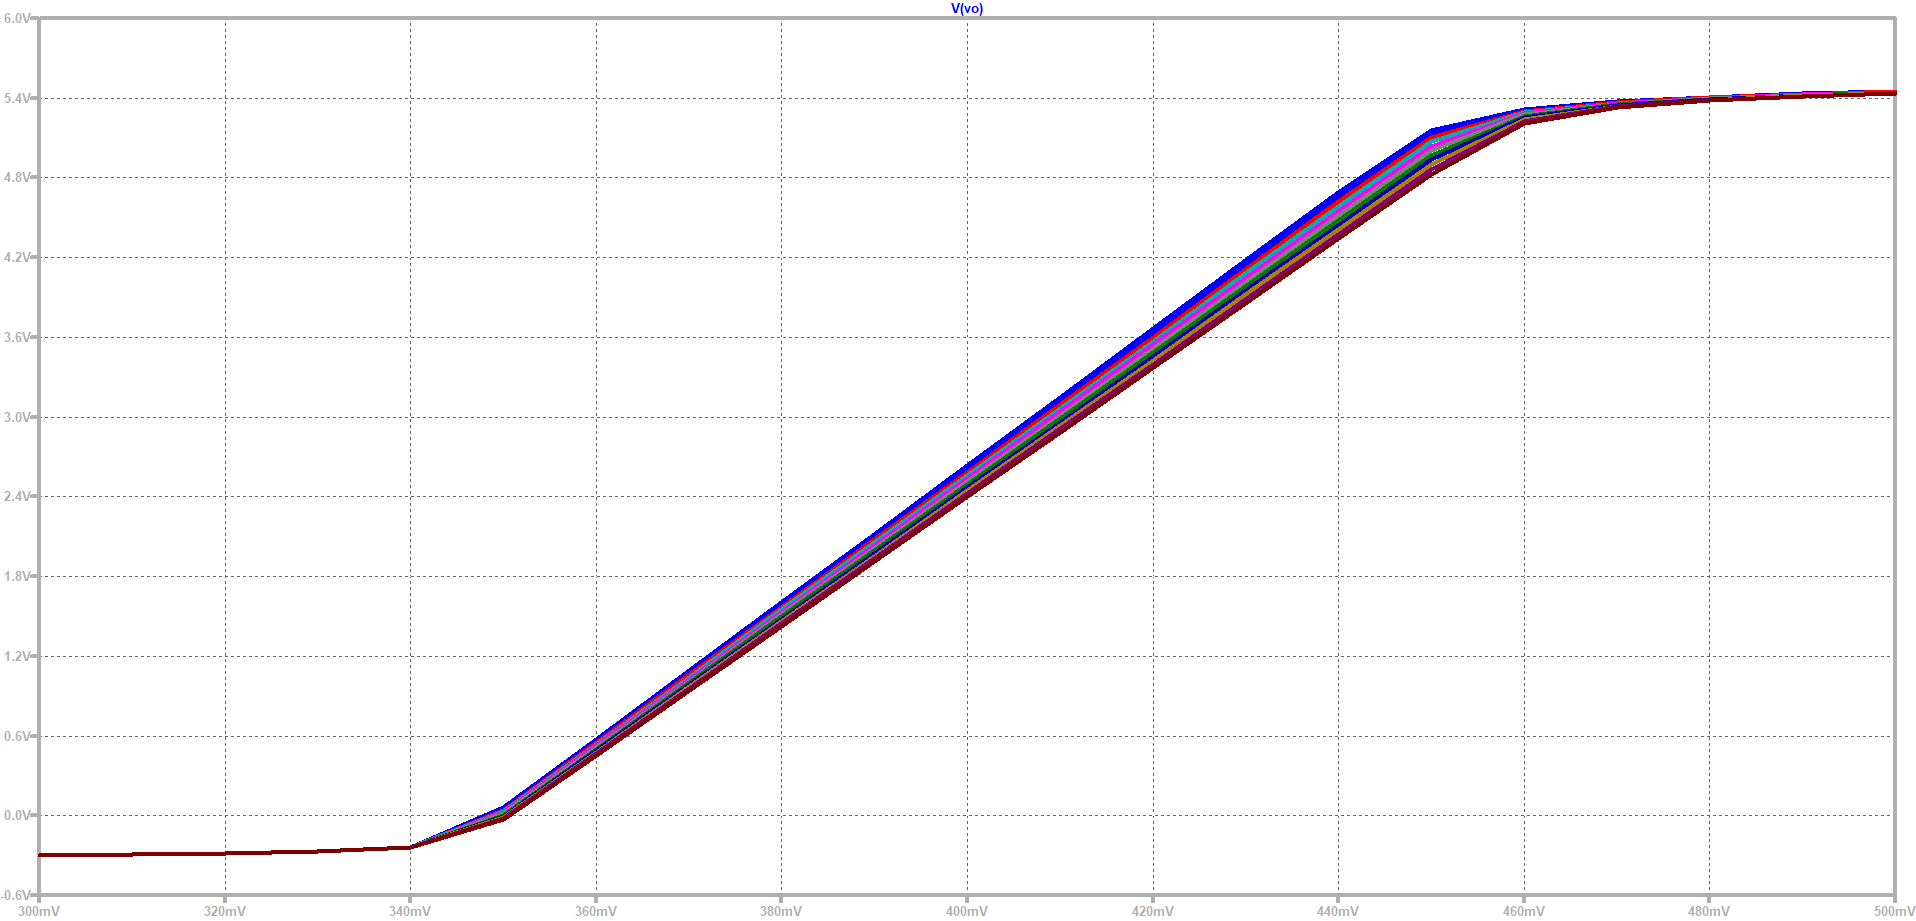
\includegraphics[width=0.99\textwidth]{Ejercicio6/Imagenes/StepR1-M1.png}
	\caption{Salida del circuito en función de la tensión del transistor variando $R_1$.}
	\label{fig:r1-M1}
\end{figure}

\begin{figure}[H]
	\centering
	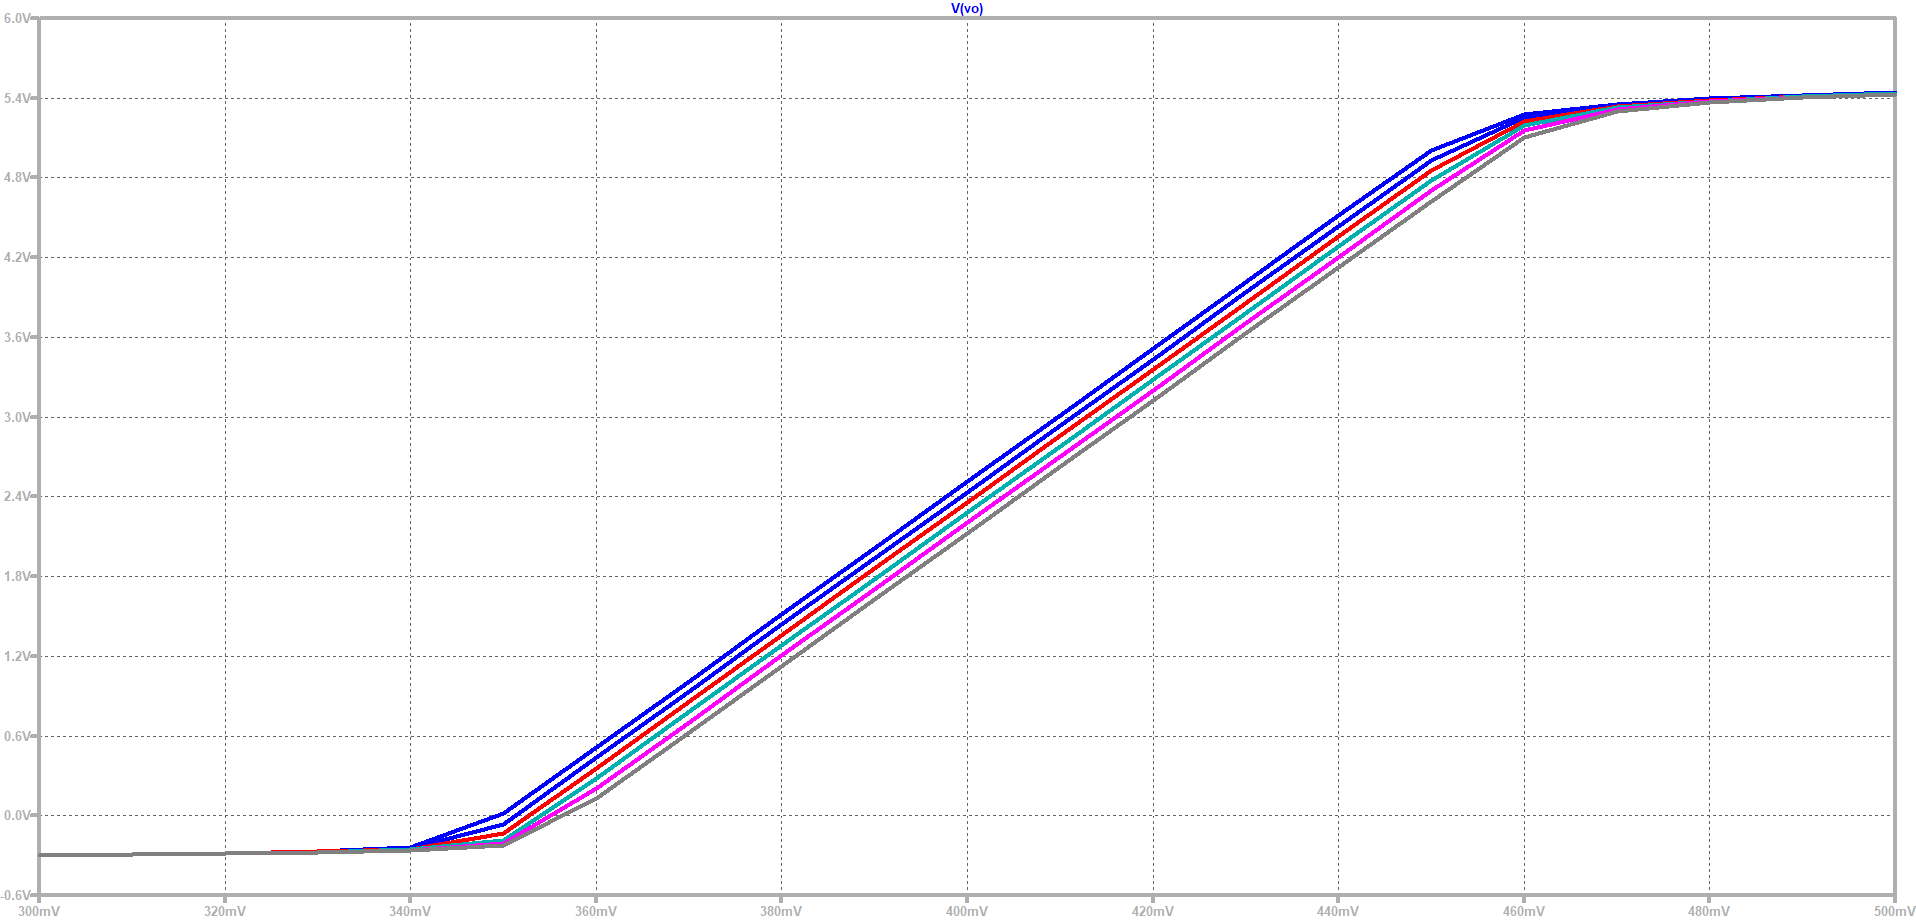
\includegraphics[width=0.99\textwidth]{Ejercicio6/Imagenes/StepR4-M1.png}
	\caption{Salida del circuito en función de la tensión del transistor variando $R_4$.}
	\label{fig:r4-M1}
\end{figure}

Ante pequeñas variaciones en $R_1$, la pendiente de la recta que describe la salida en función de la tensión del LM35 varía. De igual forma ocurre con $R_4$ y la ordenada al origen de dicha recta. Es por eso que se considera que una solución posible para esto es reemplazando tanto $R_1$ como $R_4$ por presets. De esta forma, se podrá seleccionar una valor más adecuado para obtener una salida más estable.

\subsubsection{Segundo modelo: restador e inversor}

Al igual que el circuito anterior, este está compuesto por las mismas tres etapas, con la única diferencia que se utiliza primero el amplificador restador. No se han variado ni el diodo zener utilizado, ni los modelos de operacionales utilizados, únicamente la tensión de alimentación de ambos operacionales a $12 \ V$ y $-12 \ V$.

En la primer etapa de este nuevo circuito, se suministra la tensión brindada por el transistor al borne inversor del operacional, mientras que para el no inversor, se busca reducir la tensión de $12 \ V$ de la fuente de alimentación de forma tal que la tensión en $V_2$ sea lo más próxima a $0.35 \ V$. Con esto se busca que pequeñas tensiones entren por el nodo no inversor del operacional y así evitar posibles saturaciones.

\begin{figure}[H]
\begin{center}
\begin{circuitikz}
	\node [op amp](A1){};
	\draw (A1.-) to[short] ++(-1,0) to[R, l_=$R_1$, i<_=$I_{R1}$] ++(-2,0) to[short, -o] node[ocirc,label=left:$V_{LM35}$]{} ++(-1,0);
	\draw (A1.-) node[label=south:$V^-$]{};
	\draw (A1.+) node[label=south:$V^+$]{};
	\draw (A1.+) to[short] ++(-1,0) to[R, l = $R_4$, i_>=$I_{R4}$] ++(0,-3) node[ground]{};
	\draw (A1.-) to[short] ++(0,1.5) to[R, l = $R_3$, i<=$I_{R3}$] ++(3,0) to[short] ++(0,-2);
	\draw (A1.out) to[short, -o] ++(2,0) node[ocirc,label=right:$V_{1}$]{};
	\draw (A1.+) to[short] ++(-1,0) to[R, l= $R_2$] ++(-1.5,0) to[short, -*] node[label=north:$V_2$](v2){} ++(-1,0);
	\draw (v2) to[R, l_=$R_7$, i<=$I_{R7}$] ++(-3,0) node[ocirc,label=left:$Vcc$]{};
	\draw (v2) to[R, l_=$R_8$, i_>=$I_{R8}$] ++(0,-3) node[ground]{};
	\draw (v2) to[short, i>_=$I_{R2}$] ++(1,0);
	
\end{circuitikz}
	\caption{Primera etapa del circuito.}
	\label{fig:cir1-M2}
\end{center}
\end{figure}

De la misma forma que con el primer modelo, se puede demostrar que la transferencia de esta etapa se encuentra dada por
\begin{equation}
	V_1 = \frac{R_3}{R_2} \cdot \frac{R_2 // R_4}{R_1 // R_3} \ V_2 \ - \ \frac{R_3}{R_1} V_{LM35}
	\label{equ:m2p1sinsimp}
\end{equation}

Por otro lado, planteando que
\[
	I_7 = \frac{Vcc}{R_7 + \left[ R_8 // \left( R_2 + R_4 \right) \right] }
\]

se obtiene
\[ 
	V_2 = \frac{Vcc \ \left[ R_8 // \left( R_2 + R_4 \right) \right]}{R_7 + \left[ R_8 // \left( R_2 + R_4 \right) \right]}
\]

operando de manera algebraica, se llega a 
\[ 
	V_2 = \frac{R_8 // R_7}{R_7} \cdot \frac{Vcc}{1 + \frac{R_7 R_8}{\left(R_2 + R_4 \right)\left(R_7 + R_8 \right)}}
\]

Si se consigue que 
\begin{equation}
	\frac{R_7 R_8}{\left(R_2 + R_4 \right)\left(R_7 + R_8 \right)} \approx 0
	\label{equ:condm2}
\end{equation}

se puede afirmar que  
\begin{equation}
	V_2 \approx V_{CC} \cdot \frac{R_8}{R_7 + R_8}
	\label{equ:simpm2}
\end{equation}

Utilizando (\ref{equ:simpm2}) en (\ref{equ:m2p1sinsimp}) se obtiene
\begin{equation}
	V_1 = \frac{R_3}{R_2} \cdot \frac{R_2 // R_4}{R_1 // R_3} \ \left( V_{CC} \cdot \frac{R_8}{R_7 + R_8} \right) \ - \ \frac{R_3}{R_1} V_{LM35}
	\label{equ:m2p1}
\end{equation}

Luego, para la parte del amplificador inversor, simplemente se alimentó con la tensión de salida de la etapa previa al borne inversor, mientras que se conectó el no inversor a tierra.

\begin{figure}[H]
\begin{center}
\begin{circuitikz}
	\node [op amp](A1){};
	\draw (A1.-) to[short] ++(-1,0) to[R, l = $R_5$] ++(-2,0) to[short, -o] node[ocirc,label=left:$V_{1}$](aux1){} ++(-1,0);
	\draw (aux1) to[short, i^>=$I_{R5}$] ++(,0);
	\draw (A1.-) node[label=south:$V^-$]{};
	\draw (A1.+) node[label=south:$V^+$]{};
	\draw (A1.+) to[short] ++(-1,0) node[ground]{};
	\draw (A1.-) to[short] ++(0,1.5) to[R, l = $R_6$, i<=$I_{R6}$] ++(3,0) to[short] ++(0,-2);
	\draw (A1.out) to[short, -o] ++(1,0) node[ocirc,label=right:$V_{3}$]{};
\end{circuitikz}
	\caption{Segunda etapa del circuito.}
	\label{fig:cir2-M2}
\end{center}
\end{figure}

De la misma forma que se calculó en el modelo anterior, la transferencia de esta etapa es
\begin{equation}
	V_3 = - \frac{R_6}{R_5} \ V_1
	\label{equ:m2p2}
\end{equation}

La etapa final, es decir, la protección, no cambia para este circuito. Tanto el diodo zener, como la resistencia seleccionada, son las mismas. De esta manera, con el uso de (\ref{equ:m2p1}) y (\ref{equ:m2p2}), la transferencia final queda de la forma
\begin{equation}
	V_{out} = - \frac{R_6}{R_5} \left[ \frac{R_3}{R_2} \cdot \frac{R_2 // R_4}{R_1 // R_3} \left( V_{CC} \cdot \frac{R_8}{R_7 + R_8} \right) \ - \ \frac{R_3}{R_1} V_{LM35} \right]
	\label{equ:transfm2}
\end{equation}

\begin{figure}[H]
\hspace*{-3cm} 
\begin{circuitikz}
	\node [op amp](A1){};
	\draw (A1.-) to[short] ++(-1,0) to[R, l_=$R_1$] ++(-2,0) to[short, -o] node[ocirc,label=left:$V_{LM35}$]{} ++(-1,0);
	\draw (A1.+) to[short] ++(-1,0) to[R, l = $R_4$] ++(0,-3) node[ground]{};
	\draw (A1.-) to[short] ++(0,1.5) to[R, l = $R_3$] ++(3,0) to[short] ++(0,-2);
	\draw (A1.+) to[short] ++(-1.5,0) to[R, l= $R_2$] ++(-1.5,0) node[](v2){};
	\draw (v2) to[R, l_=$R_7$] ++(-3,0) node[ocirc,label=left:$Vcc$]{};
	\draw (v2) to[R, l_=$R_8$] ++(0,-3) node[ground]{};
	
	\draw (A1.out) to[open] ++(4,-0.5) node[op amp](A2){};
	\draw (A2.-) to[short] ++(-0.5,0) to[R, l = $R_5$] ++(-1.5,0) -- (A1.out);
	\draw (A2.+) to[short] ++(-1,0) node[ground]{};
	\draw (A2.-) to[short] ++(0,1.5) to[R, l = $R_6$] ++(3,0) to[short] ++(0,-2);
	\draw (A2.out) to[short] ++(1,0) node[](v2){};
	\draw (v2) to[R, l = $R_7$] ++ (1.5,0) to[open] ++(0,-2) node[ground](gnd){};
	\draw (gnd) to[zzDo, l_= $D$] ++(0,2);
	\draw (v2) to[open] ++(1.5,0) to[short, -o] ++(1,0) node[label=right:$V_o$](){};
	
	
\end{circuitikz}	
\caption{Modelo final del circuito.}
\label{fig:cirfin-M2}
\end{figure}

Nuevamente, se imponen condiciones para obtener los valores de las resistencias, recordando que también debe cumplirse la condición impuesta en (\ref{equ:condm2}):

\begin{equation*}
\left\{
\begin{aligned}
		&	V_2 = 0.35 \ V	\\
		&	\frac{R_3}{R_1} = 10	\\
		&	\frac{R_2 // R_4}{R_1 // R_3} = 1	\\
		&	\frac{R_3}{R_2} = 10	\\
		&	\frac{R_6}{R_5} = 5
\end{aligned}
\right.
\end{equation*}

Es así que, eligiendo arbitrariamente $R_6 = 5 \ k\Omega$, $R_1 = 10 \ k\Omega$ y $R_7 = 100 \ k\Omega$ y utilizando las condiciones impuestas, se llega a: $R_2 = 10 \ k\Omega$, $R_3 = 100 \ k\Omega$, $R_4 = 100 \ k\Omega$, $R_5 = 1 \ k\Omega$ y $R_8 = \frac{700}{233} \ k\Omega \approx 3 \ k\Omega$. Se verifica ademas que con los valores seleccionados se cumpla (\ref{equ:condm2}). De esta forma 

\[
	\frac{R_7 R_8}{\left(R_2 + R_4 \right)\left(R_7 + R_8 \right)} = 0.02
\]

Nuevamente, se consigue con estos valores llegar a (\ref{equ:sistema}). Se destaca que, como la tercer etapa no ha sido alterada, sigue valiendo (\ref{equ:rzener}), por ende el valor de la resistencia, en este caso llamada $R_9$, es de $16 \ k\Omega$.

Se repite el análisis empleado para el primer circuito en LTSpice. En este caso, son las resistencias $R_5$ y $R_8$ las que resaltan.

\begin{figure}[H]
	\centering
	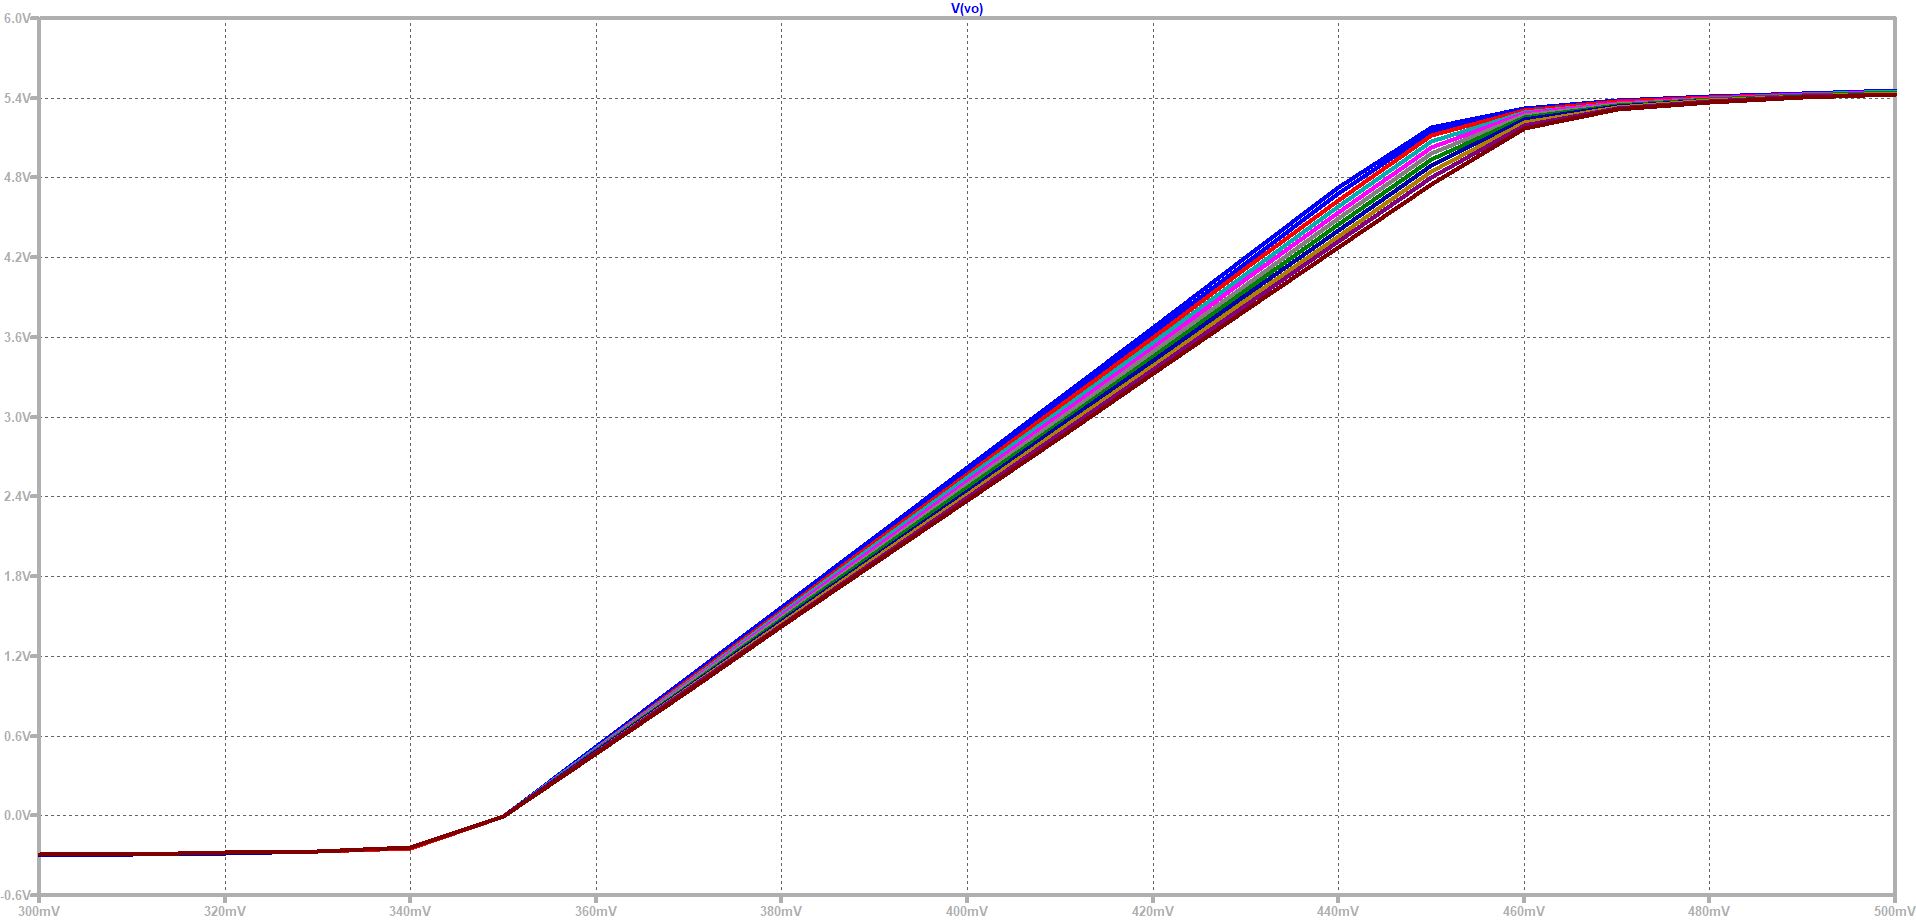
\includegraphics[width=0.99\textwidth]{Ejercicio6/Imagenes/StepR5-M2.png}
	\caption{Salida del circuito en función de la tensión del transistor variando $R_5$.}
	\label{fig:r5-M2}
\end{figure}

\begin{figure}[H]
	\centering
	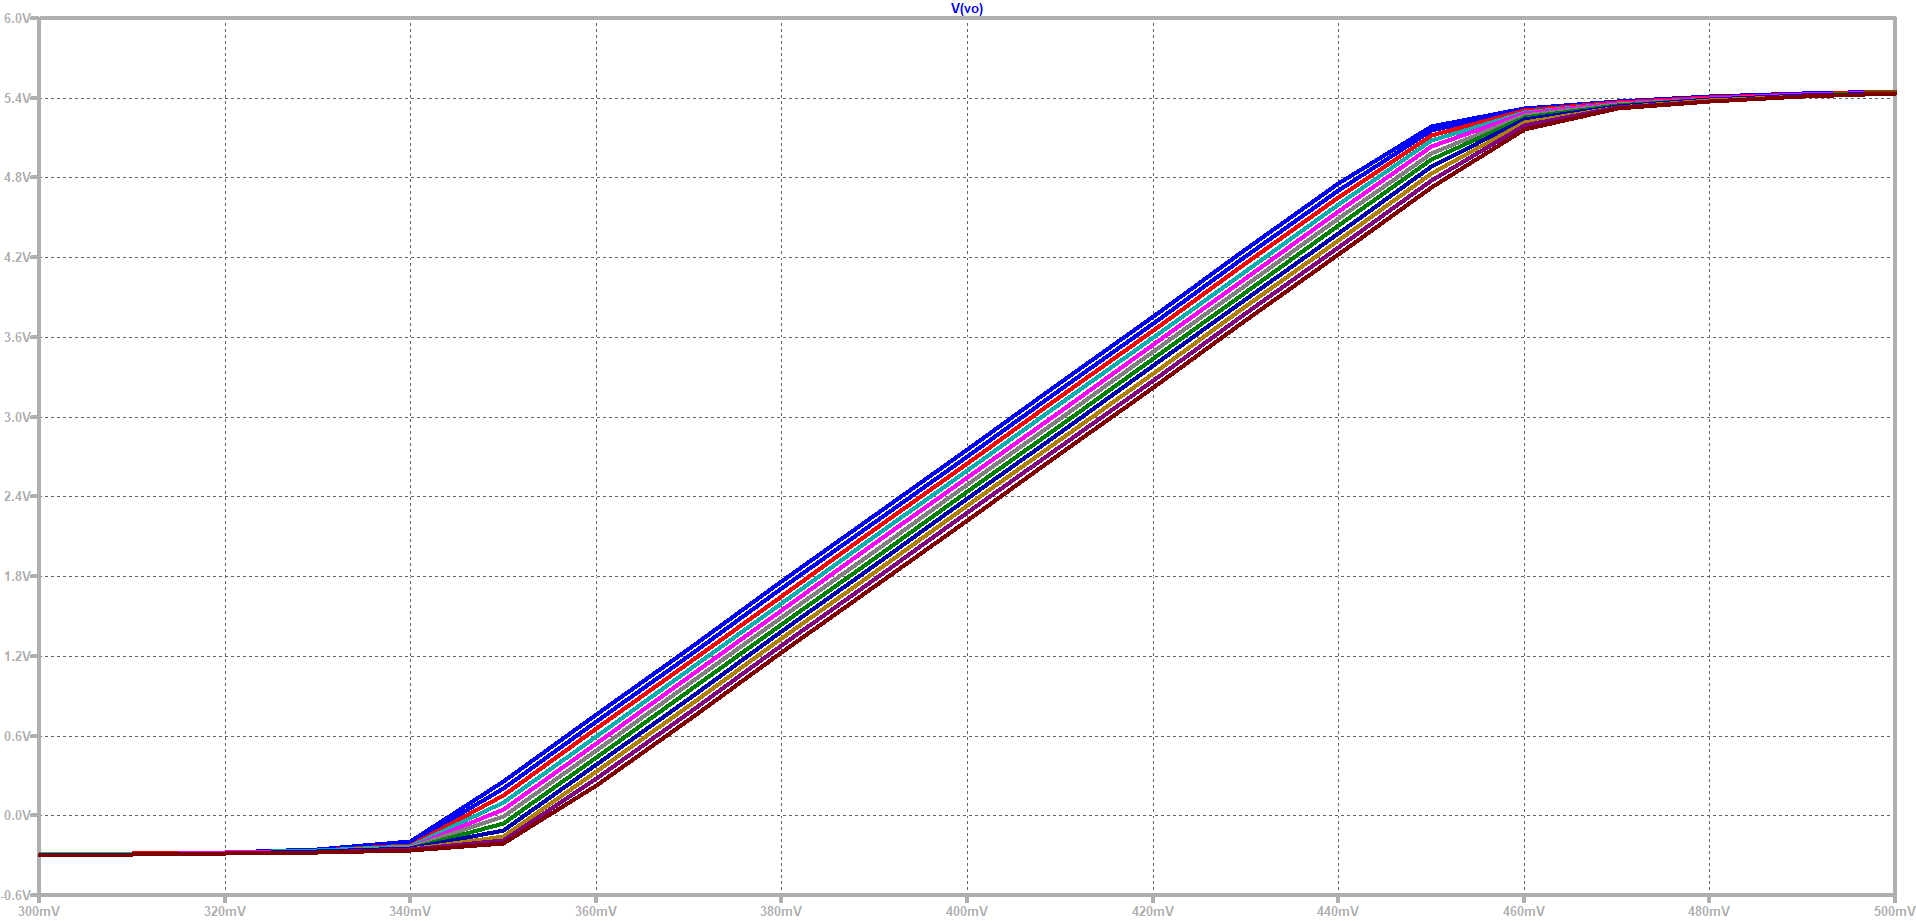
\includegraphics[width=0.99\textwidth]{Ejercicio6/Imagenes/StepR8-M2.png}
	\caption{Salida del circuito en función de la tensión del transistor variando $R_8$.}
	\label{fig:r8-M2}
\end{figure}

La pendiente de la recta que describe la salida varía con los cambios de $R_5$. Por otro lado, ordenada al origen de esta cambia con $R_4$. Nuevamente se propone como solución para esto reemplazar ambas resistencias presets.

\subsubsection{Selección del modelo más óptimo}

Se han presentado dos modelos válidos que cumplen con las especificaciones del circuito. Uno de los dos debe ser descartado. Para tomar dicha decisión se valió de la ayuda del análisis de Montecarlo, que permite realizar el programa LTSpice. Para este, se considero la tolerancia de todas las resistencias a excepción de las 4 que fueron reemplazadas por presets. Debido a que los gráficos de dicho análisis que brinda LTSpice pueden llegar a ser confusos, se decidió tomar para cada caso las curvas más alejadas de la ideal y mostrar el área encerrada entre ellas. Es así que se muestra dicho resultado en la Figura (\ref{fig:mccomp}). 

\begin{figure}[H]
\centering
\begin{subfigure}{.8\textwidth}
  \centering
  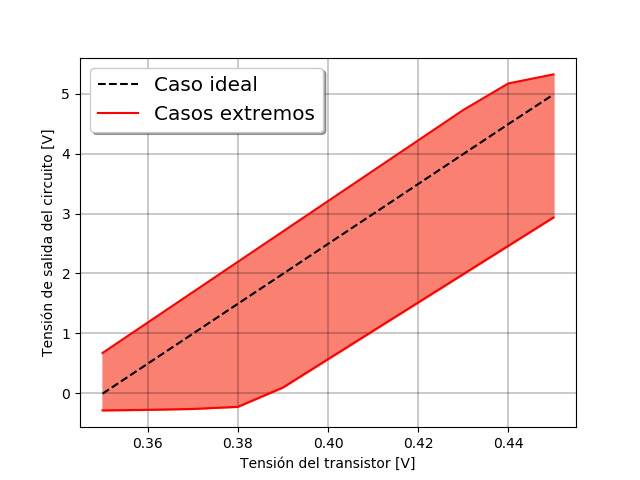
\includegraphics[width=.85\linewidth]{Ejercicio6/Imagenes/MC-1M.png}
  \caption{Primer modelo propuesto.}
  \label{fig:mcm1}
\end{subfigure}
\begin{subfigure}{\textwidth}
  \centering
  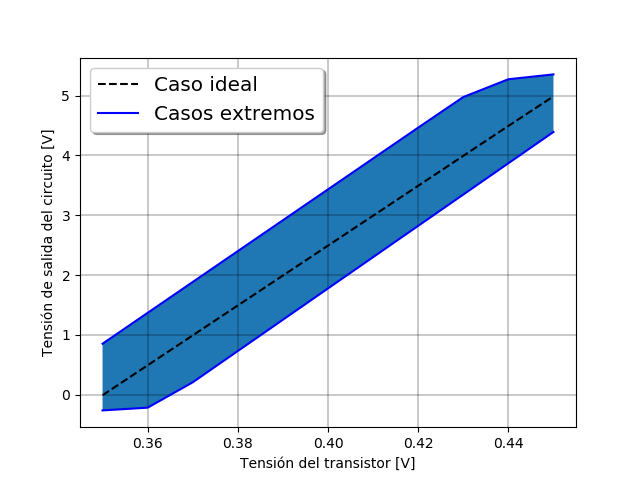
\includegraphics[width=.7\linewidth]{Ejercicio6/Imagenes/MC-2M.png}
  \caption{Segundo modelo propuesto.}
  \label{fig:mcm2}
\end{subfigure}
\caption{Comparación del los análisis de Montecarlo.}
\label{fig:mccomp}
\end{figure}

Como se observa en la Figura (\ref{fig:mccomp}), el área encerrada entre ambos extremos del primer circuito diseñado es mucho mayor que la del segundo, es decir, el primero es mucho más sensible a pequeños cambios de los componentes existentes. Fue por ello que el primer modelo propuesto fue descartado, mientras que el segundo fue aceptado. 

\begin{center}
	\textcolor{red}{\textbf{PODRÍA BUSCAR ALGUNA JUSTIFICACIÓN DE PORQUÉ DAN ASÍ LOS CIRCUITOS}}\\
	\textcolor{red}{\textbf{ESTARÍA BUENO PONER MÁS RAZONES DE PORQUÉ SE ELIGIÓ EL 2 Y NO EL 1}}
\end{center}

\subsection{Modo de uso}
%alimentacion, lectura, calibracion

Una vez analizado el circuito en LTSpice y seleccionado el modelo adecuado, se modeló este último en Altium. Como se mencionó previamente, se colocaron dos presets para poder calibrar el circuito, los cuales son representados por las resistencias $R_5$ y $R_8$ en la Figura (\ref{fig:schematic}). Se seleccionó $R_5 = 2 \ k\Omega$ y $R_8 = 5 \ k\Omega$, ya que ambos poseen la mínima resistencia entre los bornes de los extremos tal que la impedancia adecuada se encuentre dentro de este rango (se recuerda que $R_5$ debe ser próximo a $ 1 \ k\Omega$ y $R_8$ a $ 3 \ k\Omega$).

\begin{figure}[H]
	\centering
	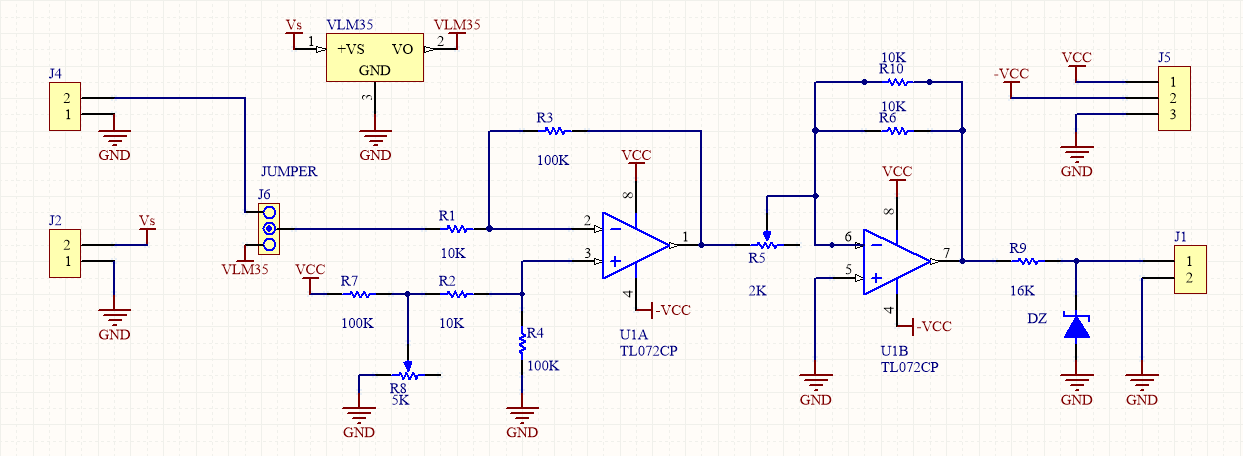
\includegraphics[width=0.99\textwidth]{Ejercicio6/Imagenes/Schematic.png}
	\caption{Esquemático del circuito en Altium.}
	\label{fig:schematic}
\end{figure}

\begin{figure}[H]
	\centering
	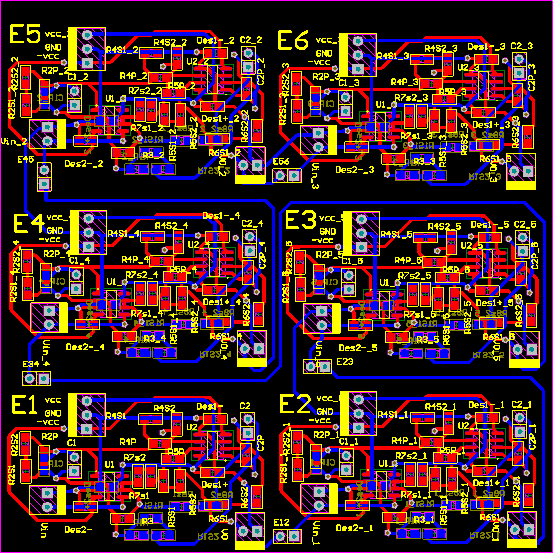
\includegraphics[width=0.8\textwidth]{Ejercicio6/Imagenes/PCB.png}
	\caption{PCB del circuito en Altium.}
	\label{fig:PCB}
\end{figure}

Para poder calibrar el circuito se colocó una entrada adicional y un jumper entre esta y el LM35, de forma que se pueda alimentar directamente al circuito con una tensión dada y calibrarlo hasta obtener la tensión de salida adecuada. Cortocircuitando el pin superior con el del medio, se habilita la entrada adicional, mientras que realizando lo mismo con el inferior y el central, se habilita el uso del transistor. Por lo tanto, para calibrarlo, la bornera $J4$ debe estar conectada con el jumper $J6$, alimentando por dicha entrada al sistema. En este caso, la bornera $J2$ queda inhabilitada y el transistor sin alimentación.

Ademas, se colocaron pines en la placa para facilitar la calibración de ambos presets. El objetivo de estos es facilitar la medición de sus tensiones al momento de ajustar las resistencias variables. Por ejemplo, se sabe que, por condiciones de fabricación, la tensión en el pin $TP8$ debe ser de $350 \ mV$. Si bien previamente se especificó que ambos operacionales deben ser alimentados con $12 \ V$ y $-12 \ V$, es posible cambiar dicho valor, dentro de las especificaciones del fabricante, y regular la resistencia $R_8$ para conseguir que la tensión en el pin $TP8$ sea la deseada. Cabe aclarar que los valores posibles que pueden tomar $R_8$ cumplen con (\ref{equ:condm2}).

Se detalla que, con el mismo objetivo que se colocó un zócalo para el amplificador operacional, se tomó la decisión de soldar tres pines hembra en lugar del transistor LM35, para poder reemplazarlo en caso de fallas.

Finalmente las borneras $J5$ y $J1$ son utilizados para alimentar a los operacionales y como salida del circuito respectivamente.

\subsection{Detalles técnicos}
Se suministró a la entrada $J4$ del circuito una rampa que cumplió la función de simular al LM35. Esta rampa barre valores desde $320 \ mV$ hasta $480 \ mV$, lo que permite que, al calibrar el sistema, se pueda observar la recta completa de salida, incluyendo las zonas donde se activa el diodo zener. De esta forma, se puede comparar la esta salida con la curva teórica mostrada en la Figura (\ref{fig:vout}).

%\begin{figure}[H]
%	\centering
%	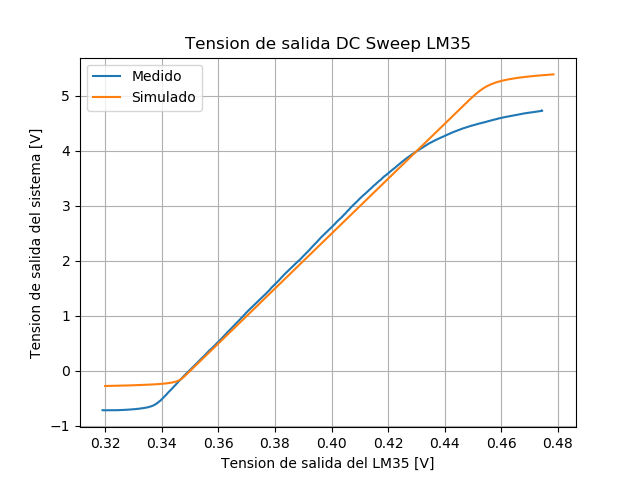
\includegraphics[width=0.8\textwidth]{Ejercicio6/Imagenes/Teovsmed.png}
%	\caption{Salida medida en comparación con la teórica.}
%	\label{fig:comp}
%\end{figure}

Si bien se buscó la mayor calibración posible, es posible observar que existe una diferencia notable entre ambas curvas. Esto se observa en la zona donde las tensiones de salida del LM35 son cercanas a $450 \ mV$.   Dicho corrimiento puede explicarse al observar nuevamente la Figura (\ref{fig:r5-M2}), ya que en la zona previamente menciona es donde se ve mayor variación. Si también se considera las tolerancias de las demás resistencias, es entendible la existencia de dicho desfasaje. Una posible solución a este problema sería reemplazar las resistencias por de metal film por resistencias SMD, las cuales poseen 1\% de tolerancia.

%Mediciones, corrientes/tensiones maximas, rango de temperatura, 

%El LM35 es un circuito integrado cuya tensión de salida varía linealmente con la temperatura. Se desea que la
%señal pueda ser adquirida por un sistema con (por ejemplo, un conversor analógico/digital) con tensión de entrada variable entre 0V y 5V .
%a. Diseñar un circuito utilizando el LM35 que adapte la señal para que pueda ser adquirida con máxima excursión para temperaturas que varíen entre 35◦C y 45◦C (35◦C ! 0V − 45◦C ! 5V ).
%b. Implementar el circuito en placa multiperforada o PCB.
%c. Diseñar un método de calibración del circuito para que se cumpla la especificación.
%d. El circuito debe contar con una protección de forma tal de que la tensión de salida no se encuentre por debajo de −1V ni por encima de 6V .
%e. Incluir en el informe un datasheet de la implementación final, incluyendo toda la información relevante.


\end{document}